\documentclass[]{informeutn}

\usepackage{array}
\usepackage{circuitikz}
\usepackage{pgfplots}
\setlength{\jot}{10pt} %interlineado en entornos aligned

% Datos del informe
\materia{Electrónica Aplicada 1}
\comision{3R2}
\titulo{Trabajo Práctico 2}
\autores{Cabaleiro Martin 404821\\Cortesini Luciano 402719\\Ernst Pedro 400624}
\fecha{21 / 5 / 2025}

\begin{document}

\maketitle

\tableofcontents
\setcounter{page}{1}
\thispagestyle{plain}


\chapter{Introducción}

En este trabajo práctico de laboratorio se llevara a cabo el análisis y construcción de una
fuente de alimentación de tensión variable. Luego se realizaran todos los ensayos pertinentes
pare verificar que la fuente cumple con las especificaciones de diseño y asegurar un correcto
funcionamiento.\\

La fuente contará con las siguientes especificaciones:
\begin{itemize}
  \item Salida regulada de $0$ a $30\V$.
  \item Corriente máxima de $1.5\A$.
\end{itemize}

\chapter{Planteamiento e introducción teórica}

El siguiente diagrame en bloques sintetiza las distintas etapas de la fuente, Desde la entrada de
$220V$ en CA hasta llegar a la tension en CC a la salida.

\begin{figure}[h]
  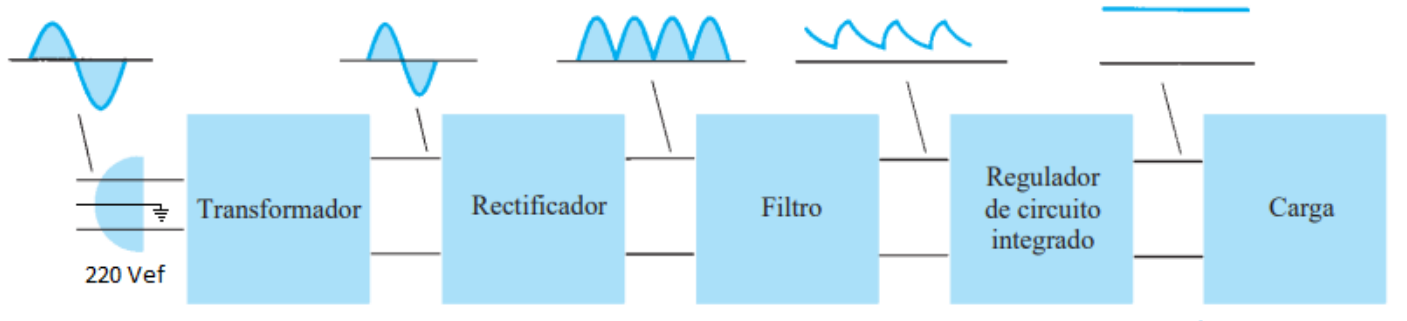
\includegraphics[width=0.95\textwidth]{images/diagramaBloques.png}
  \caption{Diagrama en bloques}
\end{figure}

A contunuación, se explica detaladamente cada uno de estos bloques.

\section{Transformador}

El transformador tiene dos funciones:
\begin{itemize}
  \item Aislar galvánicamente el circuito de la red electrica.
  \item Reducir la tension de entrada al valor necesario para la fuente.
\end{itemize}

\begin{circuitikz}
  \draw (0,0) to [sV] ++(0,2) -- ++(1,0)
  node[transformer core, circuitikz/inductors/coils=6,
  anchor=A1](T){};
  \draw (T.A2) -| (0,0);
  \draw (T-L2.midtap) to[short, *-] (T.B1 |- T-L2.midtap);
  \draw (T.B2) to[short, -o] ++(1.2,0);
  \draw (T.B1) ++(0.6,-0.55) node[spdt, rotate=180](SW){} ;
  \draw (T.B1) -| (SW.out 2);
  \draw (T-L2.midtap) -| (SW.out 1);
  \node [ocirc] at (SW.in){};
\end{circuitikz}

En nuestro caso particular, utilizaremos un transformador con punto medio, que a travez de una llave selectora
nos permitirá elegir entre una tension de entrada a nuestra fuente de $12$ o $24\V$.

\hspace{5mm}

\begin{figure}[h]
  \centering
  \begin{circuitikz}
    \draw (0,2) to[short, o-] ++(1,0)
    node[transformer core, circuitikz/inductors/coils=6,
    anchor=A1](T){};
    \draw (T.A2) to[short, -o] ++(-1,0);
    \node at ($($(T.A1)!0.5!(T.A2)$) +(-1,0)$) []{$220\V$};

    \draw (T-L2.midtap) to[short, *-] (T.B1 |- T-L2.midtap);
    \draw (T.B2) to[short, -o] ++(1.2,0);
    \draw (T.B1) ++(0.6,-0.54) node[spdt, rotate=180](SW){} ;
    \draw (T.B1) -| (SW.out 2);
    \draw (T-L2.midtap) -| (SW.out 1);
    \node [ocirc] at (SW.in){};
    \node at ($(SW.in)!0.5!(SW.in |- T.B2)$) []{$12/24\V$};

  \end{circuitikz}
  \caption{Transformador con punto medio}
\end{figure}

En la sección \ref{sec:filtro} analizaremos el por que de esta decisión.

\newpage
\section{Rectificador}
Tiene la función de convertir la tensión alterna en una pulsante.

En nuestro caso utilizaremos un puente rectificador compuesto por diodos 1N5407.

\vspace{5mm}

\begin{figure}[h]
  \centering
  \begin{circuitikz} [circuitikz/diodes/scale=0.7]
    \draw (0,0) coordinate(top bridge) to [full diode, *-*, l={\footnotesize D2}] ++(1.5,-1.5) coordinate(right bridge)
    to [full diode, *-*, invert, l={\footnotesize D4}] ++(-1.5,-1.5) coordinate (bottom bridge)
    to [full diode, *-*, invert, l={\footnotesize D3}] ++(-1.5,1.5) coordinate (left bridge)
    to [full diode, *-*, l={\footnotesize D1}] (0,0);

    \draw (top bridge) to[short, -o] ++(-2.5,0) coordinate(inA);
    \draw (bottom bridge) to[short, -o] ++(-2.5,0) coordinate(inB);
    \draw (right bridge) to[short, -o] ++(1,0) coordinate(outA);
    \draw (left bridge) to[short] ++(0,-2) to[short, -o] ++(4,0) coordinate(outB);

    \node at ($(inA)!0.5!(inB)$) []{$v_{in}$};
    \node at ($(outA)!0.5!(outB)$) []{$v_{out}$};

  \end{circuitikz}
  \caption{Puente de diodos}
\end{figure}

Este circuito es un rectificador de onda completa, es decir que convierte todos los semiciclos en positivos.

\begin{figure}[h]
  \begin{minipage}[t][5cm][c]{0.5 \textwidth}
    \centering
    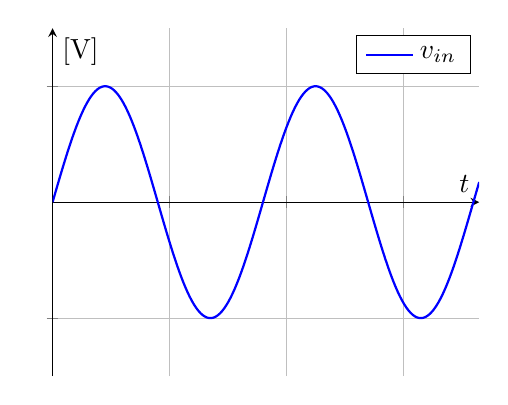
\begin{tikzpicture}
      \begin{axis}[
          axis lines=middle,
          xlabel={$t$},
          ylabel={[V]},
          xticklabels={},
          yticklabels={},
          domain=0:730,
          samples=200,
          grid=both,
          width=7cm,
          height=6cm,
          ymin=-3, ymax=3,
          xmin=0, xmax=730,
        ]
        \addplot[blue, thick] {2*sin(x)};
        \addlegendentry{$v_{in}$}
      \end{axis}
    \end{tikzpicture}
  \end{minipage}
  \begin{minipage}[t][5cm][c]{0.5 \textwidth}
    \centering
    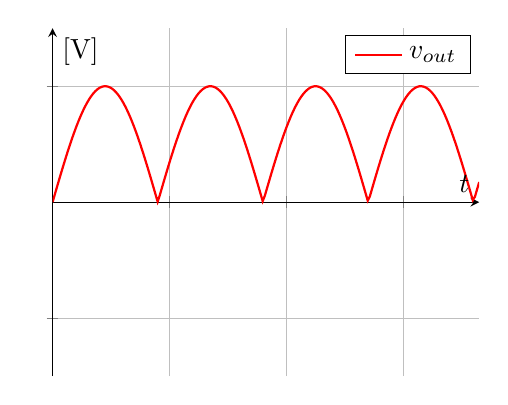
\begin{tikzpicture}
      \begin{axis}[
          axis lines=middle,
          xlabel={$t$},
          xticklabels={},
          yticklabels={},
          ylabel={[V]},
          domain=0:730,
          samples=200,
          grid=both,
          width=7cm,
          height=6cm,
          ymin=-3, ymax=3,
          xmin=0, xmax=730,
        ]
        \addplot[red, thick] {abs(2*sin(x))};
        \addlegendentry{$v_{out}$}
      \end{axis}
    \end{tikzpicture}
  \end{minipage}
  \caption{señales de entrada y salida}
\end{figure}

Para comprender su funcionamiento, podemos analizar por separado el comportamiento del circuito durante el semiciclo positivo y el
semiciclo negativo, considerando que hay una carga conectada.

Durante el semiciclo positivo, el terminal superior de la entrada presenta un mayor potencial que el inferior. En esta condición, los diodos
D2 y D3 se encuentran polarizados en directa, mientras que D1 y D4 están polarizados en inversa. La corriente fluye desde el terminal
superior, atravesando el diodo D2, pasando por la carga, luego por el diodo D3, y finalmente hacia el terminal inferior de la entrada.

Durante el semiciclo negativo, el terminal inferior de la entrada se encuentra a mayor potencial que el superior. En este caso, los diodos
D1 y D4 quedan polarizados en directa, y D2 y D3 en inversa. La corriente fluye desde el terminal inferior, pasando por el diodo D4,
atravesando la carga en el mismo sentido que en el semiciclo positivo, y continuando por el diodo D1 hasta llegar al terminal superior.

Como resultado, en ambos semiciclos la corriente atraviesa la carga en la misma dirección, lo que permite obtener una señal rectificada
de onda completa.

\begin{figure}[h]
  \begin{minipage}[t][8cm][c]{0.5 \textwidth}
    \centering
    \begin{circuitikz} [circuitikz/diodes/scale=0.7, american]
      \draw (0,0) coordinate(top bridge) to [full diode, *-*, l={\footnotesize D2}, f={i}] ++(2,-2) coordinate(right bridge)
      to [full diode, *-*, invert, l={\footnotesize D4}] ++(-2,-2) coordinate (bottom bridge)
      to [full diode, *-*, invert, l={\footnotesize D3}, f_<=i ] ++(-2,2) coordinate (left bridge)
      to [full diode, *-*, l={\footnotesize D1}] (0,0);

      \draw (top bridge) to[short, -o, f_<={i},] ++(-3.5,0) coordinate(inA);
      \draw (bottom bridge) to[short, -o, f=i] ++(-3.5,0) coordinate(inB);
      \draw (right bridge) to[short] ++(1,0) coordinate(outA);
      \draw (left bridge)to[short] ++(-0.3,0) to[short] ++(0,-3) to[short, f_<=i] ++(5.3,0) coordinate(outB);

      \draw (outA) to[R, v_=$v_L$, f=i] (outB);

      \node at ($(inA)!0.5!(inB)$) []{$v_{in}$};

      \node at ($(inA) +(-0.4,0)$) []{+};
      \node at ($(inB) +(-0.4,0)$) []{-};

    \end{circuitikz}
    \caption{Semiciclo positivo}
  \end{minipage}
  \begin{minipage}[t][8cm][c]{0.5 \textwidth}
    \centering
    \begin{circuitikz} [circuitikz/diodes/scale=0.7, american]
      \draw (0,0) coordinate(top bridge) to [full diode, *-*, l={\footnotesize D2}] ++(2,-2) coordinate(right bridge)
      to [full diode, *-*, invert, l={\footnotesize D4}, f<={i}] ++(-2,-2) coordinate (bottom bridge)
      to [full diode, *-*, invert, l={\footnotesize D3}] ++(-2,2) coordinate (left bridge)
      to [full diode, *-*, l={\footnotesize D1}, f>_={i}] (0,0);

      \draw (top bridge) to[short, -o, f_=i] ++(-3.5,0) coordinate(inA);
      \draw (bottom bridge) to[short, -o, f<=i] ++(-3.5,0) coordinate(inB);
      \draw (right bridge) to[short] ++(1,0) coordinate(outA);
      \draw (left bridge)to[short] ++(-0.3,0) to[short] ++(0,-3) to[short, f_<=i] ++(5.3,0) coordinate(outB);

      \draw (outA) to[R, v_=$v_L$, f = i] (outB);

      \node at ($(inA)!0.5!(inB)$) []{$v_{in}$};

      \node at ($(inA) +(-0.4,0)$) []{-};
      \node at ($(inB) +(-0.4,0)$) []{+};

    \end{circuitikz}
    \caption{Semiciclo negativo}
  \end{minipage}
\end{figure}

\subsection{Elección de los diodos}

Para dimensionar correctamente los diodos del puente, partimos de que la fuente debe entregar 1,5\,A continuos a la carga. Sin embargo, cada
par de diodos sólo conduce durante un semiciclo (50\,\% del tiempo), de modo que la \emph{corriente media} que atraviesa cada “rama” del
puente es:


\begin{equation}
I_{\mathrm{media\;por\;rama}} = 1{,}5\;\mathrm{A} \times 0{,}5 = 0{,}75\;\mathrm{A}.
\end{equation}

Si usásemos diodos de la serie 1N4001–1N4007 (1\,A de corriente continua), tendríamos un margen de sólo $0{,}25\A$ sobre esa
corriente media. Además, el regulador LM317, aunque nominalmente entrega 1,5\,A, puede generar picos de hasta 2,1\,A antes
de activar su protección interna, y esos picos también cruzan el puente de diodos.

Como los diodos de 2\,A no son habituales, elegimos la serie 1N5400–1N5408 (3\,A de corriente continua), que ofrece:

\begin{itemize}
    \item Suficiente margen sobre los 0,75\,A medios de cada rama.
    \item Capacidad de soportar picos transitorios sin acercarse a su límite máximo.
\end{itemize}

De este modo garantizamos un funcionamiento y seguro, minimizando el riesgo de sobrecalentamiento o daño por sobrecorriente.

\section{Filtro}
\label{sec:filtro}
La onda pulsante a la salida del rectificador no es apta para alimentar
equipos electrónicos por ello se le agrega un capacitor de filtro para
alizarla, la formula para calcular el mismo es:

\begin{equation}
  C=\frac{I_L}{2 \cdot f_{salida} \cdot \Delta V}
  \label{eq:filtro}
\end{equation}

formula extraida del libro Amplificadores Operacionales y Circuitos Integrados Lineales Coughlin-Driscol. Esta formula predice
muy bien el riple obtenido experimentalmente.
Siendo $\Delta V$ la tension pico a pico del ripple

En nuestro caso, utilizaremos un capacitor de $3300\uF$. Podemos calcular el valor esperado de $\Delta V$ despejando de \ref{eq:filtro}.

\begin{equation}
  \begin{aligned}
    \Delta V&=\frac{I_L}{2 \cdot f_{salida} \cdot C}\\
    \Delta V&=\frac{1{,}5\A}{2 \cdot 100\Hz \cdot 3300\uF}\\
    \Delta V&= 2{,}272 \V
  \end{aligned}
\end{equation}

\section{Regulador de circuito integrado}
La funcióones del regualdor son:

\begin{itemize}
  \item Mantener estable la tensión de salida de la fuente sin importar las variaciones tanto de la corriente de carga como de la red electrica.
  \item Reducir el ripple en un orden de mil veces.
\end{itemize}

\chapter{Ensayos y mediciones}

\section{Medición de ripple (sin regulador)}

Para poder realizar las siguiente mediciones en este primer ensayo, previamente se realizo en la placa la soldadura del puente diodo y el filtro.

\subsection{En el filtro capacitivo y determinación de parámetros.}

Se tomaran medidas de la tension tanto en el punto bajo como en el punto alto del transformador variando la
corriente desde el vacio (0 A) hasta llegar a plena carga (1,5 A). Con las mediciones vamos a poder calcular los siguientes tres factores:
Regulacion de voltaje, resistencia variable y factor de ripple.\\

\subsubsection{Punto bajo}

\begin{table}[H]
  \centering
  \begin{tabular}{|c|c|}
    \hline
    $V_{vacio}$ & 17,71 V \\ \hline
    $V_{0,5 A}$ & 15,80 V \\ \hline
    $V_{0,75 A}$ & 15,27 V \\ \hline    
    $V_{1 A}$ & 14,63 V \\ \hline
    $V_{1,25 A}$ & 14,10 V \\ \hline
    $V_{PlenaCarga}$ & 13,69 V \\ \hline
  \end{tabular}
  \caption{Mediciones en el punto bajo}
\end{table}


\begin{figure}[H]
  \centering
  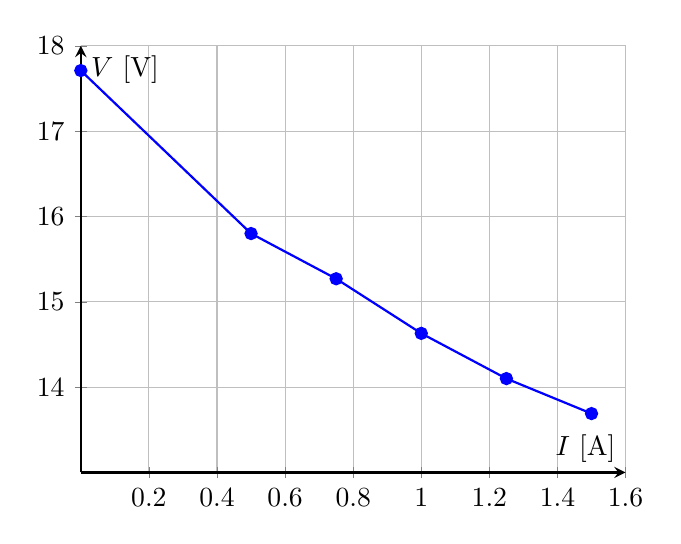
\begin{tikzpicture}
    \begin{axis}[
      axis lines = middle,
      xlabel = {$I$ [A]},
      ylabel = {$V$ [V]},
      domain = 0:1.5,
      samples = 200,
      grid = both,
      width=8.5cm,
      height=7cm,
      xmin = 0, xmax= 1.6,
      ymin = 13, ymax = 18,
      thick
      ]
      \addplot[blue, mark=*] coordinates {
            (0, 17.71)
            (0.5, 15.80)
            (0.75, 15.27)
            (1, 14.63)
            (1.25, 14.10)
            (1.5, 13.69)
      };
    \end{axis}
  \end{tikzpicture}
  \caption{Vout vs Iout punto bajo}
\end{figure}

\subsubsection{Punto alto}

\begin{table}[H]
  \centering
  \begin{tabular}{|c|c|}
    \hline
    $V_{vacio}$ & 36,86 V \\ \hline
    $V_{0,5 A}$ & 31,89 V \\ \hline
    $V_{0,75 A}$ & 31,05 V \\ \hline    
    $V_{1 A}$ & 29,83 V \\ \hline
    $V_{1,25 A}$ & 28,55 V \\ \hline
    $V_{PlenaCarga}$ & 27,47 V \\ \hline
  \end{tabular}
  \caption{Mediciones en el punto alto}
\end{table}

\begin{figure}[H]
  \centering
  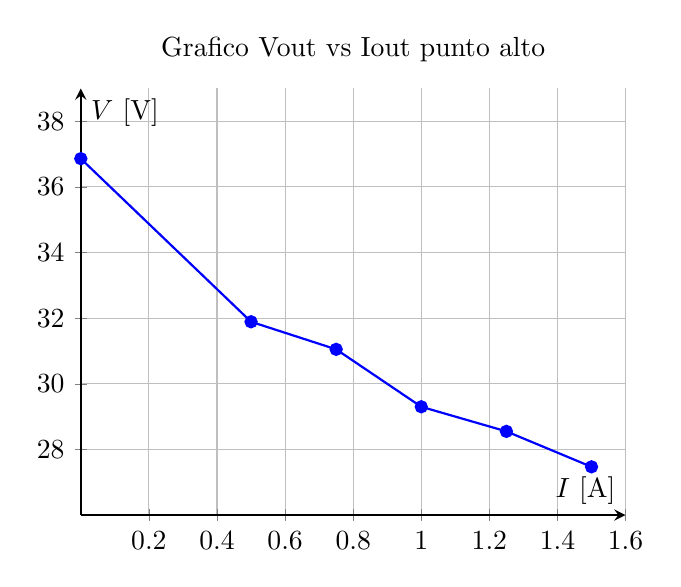
\begin{tikzpicture}
    \begin{axis}[
      axis lines = middle,
      xlabel = {$I$ [A]},
      ylabel = {$V$ [V]},
      domain = 0:1.5,
      samples = 200,
      grid = both,
      width=8.5cm,
      height=7cm,
      title = {Grafico Vout vs Iout punto alto},
      xmin = 0, xmax= 1.6,
      ymin = 26, ymax = 39,
      thick
      ]
      \addplot[blue, mark=*] coordinates {
            (0, 36.86)
            (0.5, 31.89)
            (0.75, 31.05)
            (1, 29.3)
            (1.25, 28.55)
            (1.5, 27.47)
      };
    \end{axis}
  \end{tikzpicture}
\end{figure}

\subsection{Determinación de resistencia interna del transformador más la de los diodos.}

\subsubsection{Punto bajo}

Para calcular la regulacion de voltaje se utiliza la siguiente formula:

\begin{equation}
  \begin{aligned}
    RV &= \dfrac{V_{vacio} - V_{PlenaCarga}}{V_{PlenaCarga}} 100\percent \\
    RV &= \dfrac{17,71\V - 13,69\V}{13,69\V} 100\percent = 29,36\percent
  \end{aligned}
\end{equation}

La resistencia interna esta dada por:

\begin{equation}
  \begin{aligned}
    R_{int} &= \dfrac{V_{PlenaCarga} - V_{vacio}}{-I_{carga}}\\
    R_{int} &= \dfrac{13,69\V - 17,71\V}{-1,5\A} = 2,68\ohm
  \end{aligned}
\end{equation}

Ahora mediremos el voltaje del ripple tanto con multimetro true RMS, como en el osciloscopio:

\begin{equation}
  V_{RippleMultimetro} = 908 mV
\end{equation}
\begin{equation}
  V_{RippleOsciloscopio} = 972 mV
\end{equation}
\begin{equation}
  V_{PicoaPico} = 2,75 V
\end{equation}

Factor de ripple:

\begin{equation}
  \begin{aligned}
    F_R &= \dfrac{V_{eficaz}}{V_{PlenaCarga}} 100\percent\\
    F_R &= \dfrac{908 mV}{13,69 V} 100\percent\\
    F_R &= 6,6325\percent
  \end{aligned}
\end{equation}

\subsubsection{Punto alto}
Para el punto alto repetiremos las formulas del punto bajo cambiando por los valores correspondientes: \\

Regulacion de voltaje:

\begin{equation}
  RV = \dfrac{36,68\V - 27,43\V}{27,43\A} 100\percent = 33,72\percent
\end{equation}

Resistencia interna:

\begin{equation}
  R_{int} = \dfrac{27,43\V - 36,68\V}{-1,5\A} = 6,16\ohm
\end{equation}

Ripple:

\begin{equation}
  V_{RippleMultimetro} = 0,83 V
\end{equation}

\begin{equation}
  V_{RippleOsciloscopio} = 0,88 V
\end{equation}

\begin{equation}
  V_{PicoaPico} = 2,5 V
\end{equation}

Factor de rippple:

\begin{equation}
  \begin{aligned}
    F_R &= \dfrac{0,83 V}{27,43 V} 100\percent\\
    F_R &= 3,0258
  \end{aligned}
\end{equation}


\section{Mediciones finales (con regulador)}

A continuación, se llevarán a cabo una serie de mediciones destinadas a verificar el correcto funcionamiento del regulador LM317 en la
fuente montada. Estas pruebas incluyen la medición de caída de tensión y corriente para alcanzar su potencia máxima, análisis de la
regulación de voltaje tanto en vacío como a plena carga, evaluación del ripple mediante osciloscopio y cálculo de su factor, así como la
medición de temperatura en el encapsulado del regulador para estimar su temperatura interna. Estas mediciones permitirán validar el
desempeño eléctrico y térmico del circuito en condiciones reales de operación.

\begin{figure}[h]
  \centering
  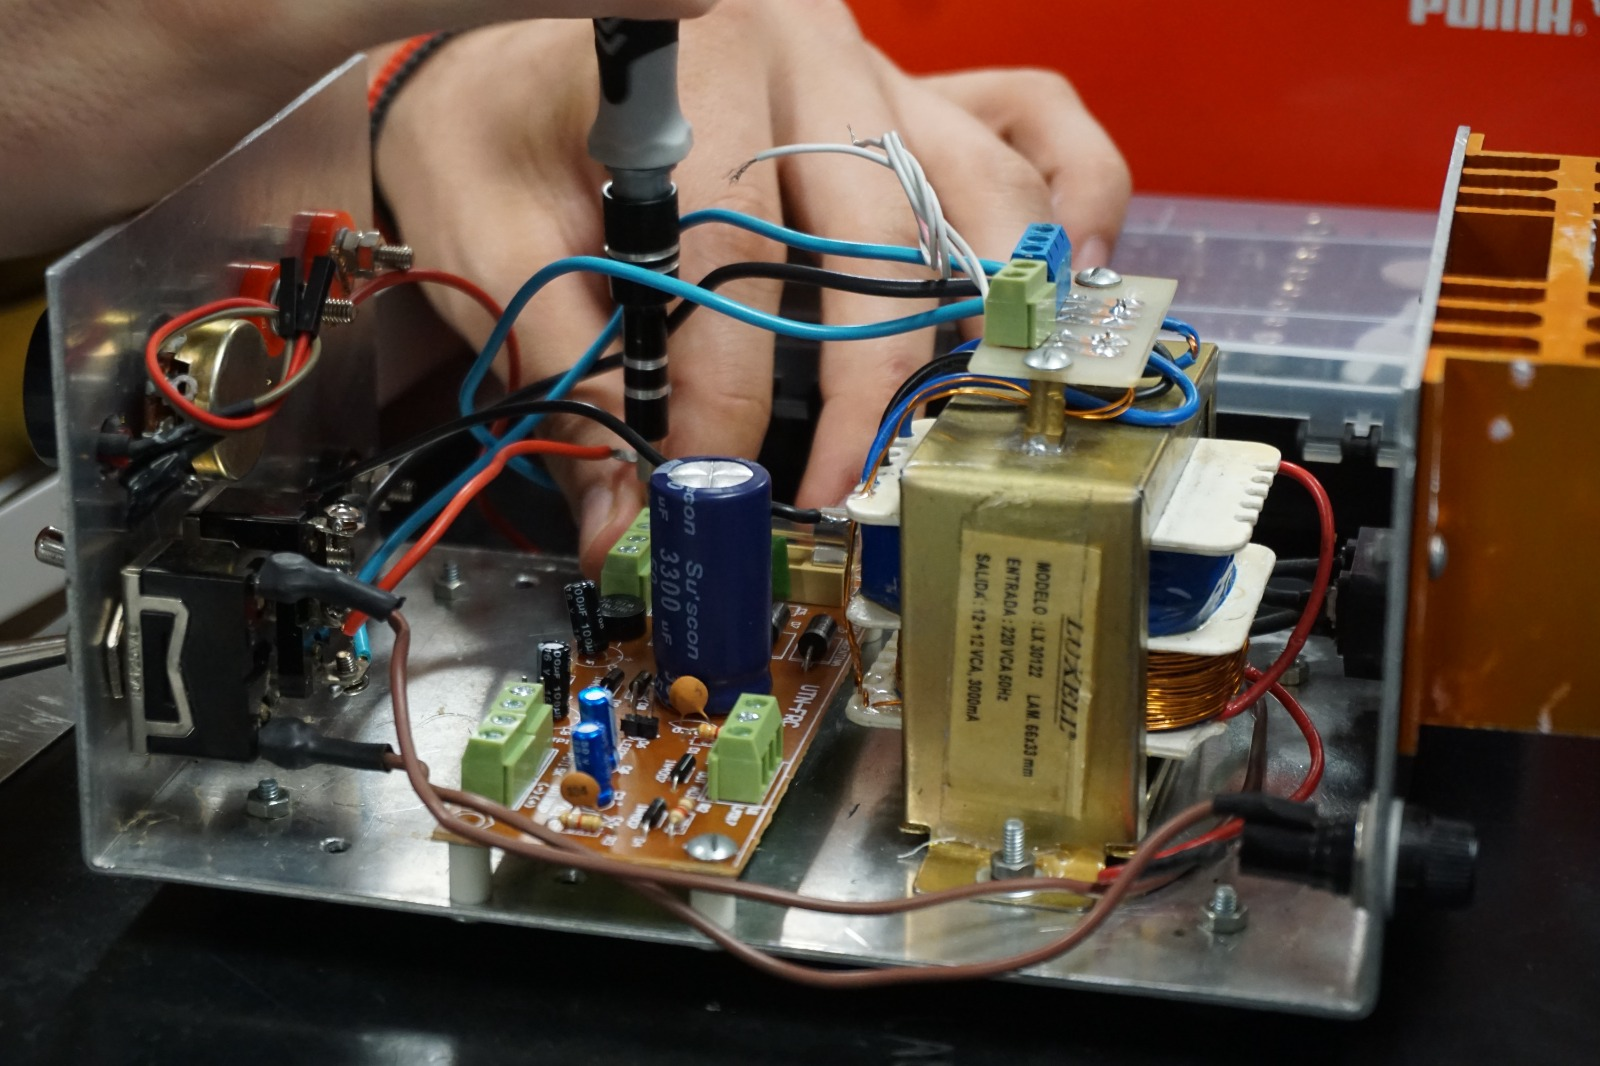
\includegraphics[width=0.70\textwidth]{images/placaMontada.png}
\end{figure}

\subsection{Regulación de voltaje.}

\begin{table}[H]
  \centering
  \begin{tabular}{|c|c|}
    \hline
    $V_{vacio}$ & 16,92 V \\ \hline
    $V_{PlenaCarga}$ & 16,29 V \\ \hline
  \end{tabular}
\end{table}

\begin{equation}
  \begin{aligned}
    RV &= \dfrac{16,92 - 16,29}{16,29} 100\percent\\
    RV &= 3,867
  \end{aligned}
\end{equation}

\subsection{Factor de ripple.}

\begin{equation}
  V_{RippleEficaz} = 353,55 . 10^{-6} V = 353,5 uV 
\end{equation}

\begin{equation}
  \begin{aligned}
    F_R &= \dfrac{353,5 uV}{16,29 V} 100\percent\\
    F_R &= 2,1703 . 10^{-3}\percent
  \end{aligned}
\end{equation}

\begin{figure}[H]
  \centering
  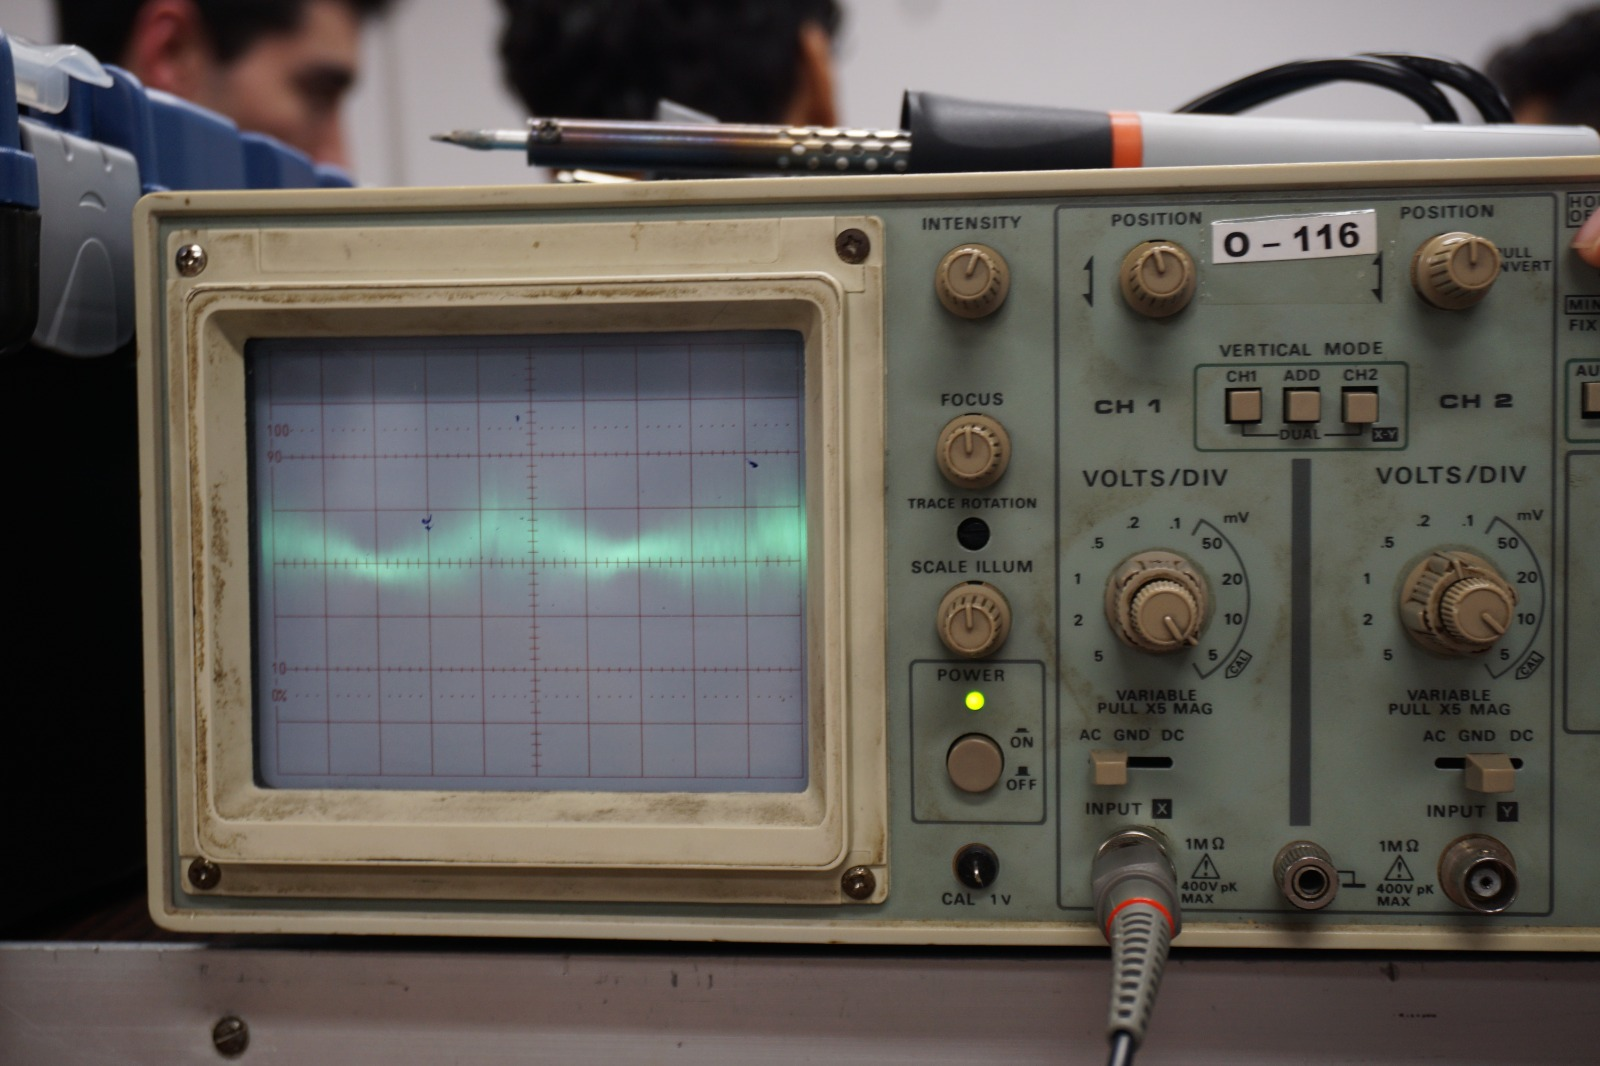
\includegraphics[width=0.70\textwidth]{images/medicionRipple.png}
  \caption{Visualizacion de riple en osciloscopio}
\end{figure}


\subsection{Cálculo de temperatura de juntura.}

\begin{figure}[H]
  \centering
  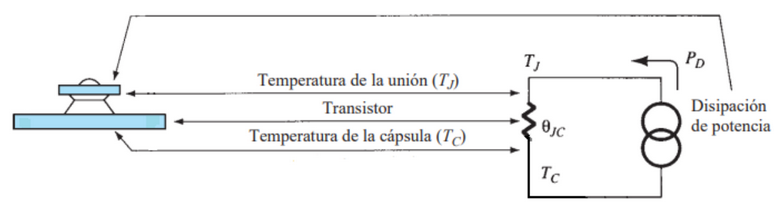
\includegraphics[width=0.95\textwidth]{images/calculoTemperatura.png}
  \caption{Calculo de la temperatura}
\end{figure}

\begin{equation}
  T_J - T_C = \theta_{JC} \times P_D \quad \Rightarrow \quad T_J = \theta_{JC} \times P_D + T_C
\end{equation}

Siendo: \\

$\theta_{jc} = 5\dfrac{\circ C}{W} $ : Resistencia termica de la juntura \\

$T_J = 135 \circ C$ : Temperatura de la juntura \\

$135 \circ C = (5 \dfrac{\circ C}{W} 15,19 W) + T_C $

$135 \circ C - 75 \circ C = T_C$

$T_C = 60 \circ C$ : Temperatura del chip

\begin{figure}[H]
  \centering
  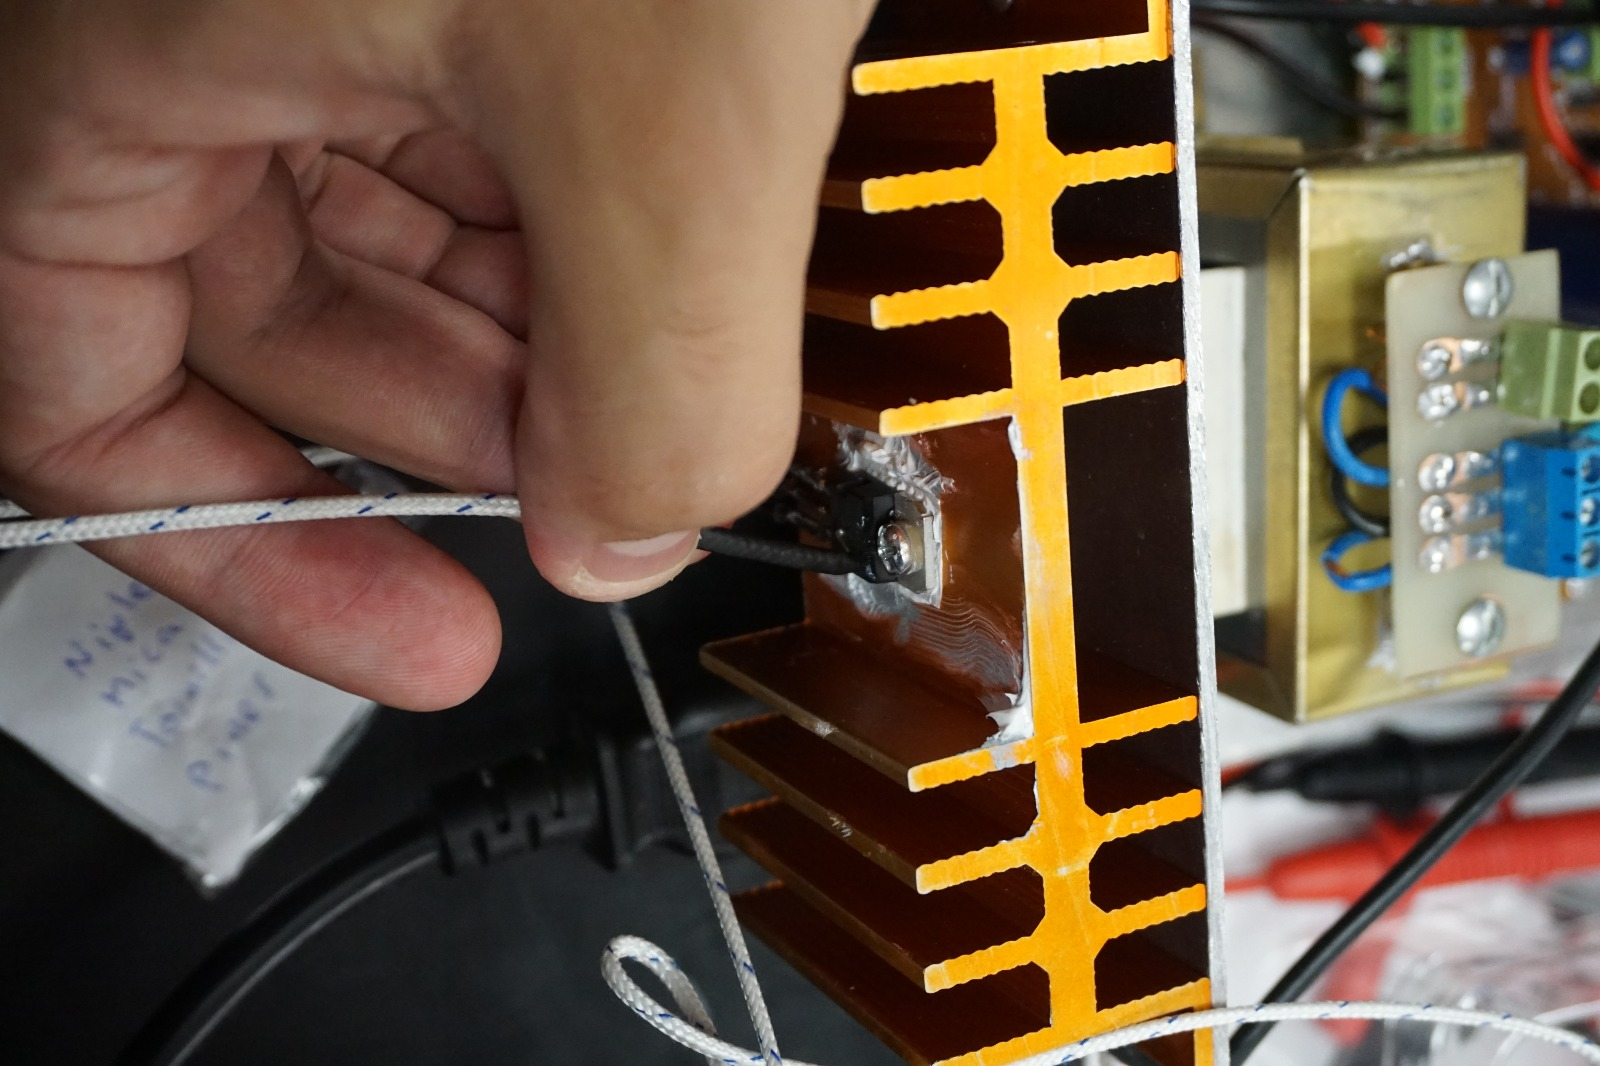
\includegraphics[width=0.70\textwidth]{images/medicionTemperatura.png}
  \caption{Medicion de la tempera en LM317}
\end{figure}


\chapter{Conclusiones}


\end{document}
